\documentclass[11pt]{article}
\usepackage[margin=0.82in]{geometry}
\usepackage{amsmath,amssymb,booktabs,graphicx,float,longtable,pgfplots,listings,xcolor}
\pgfplotsset{compat=1.18}
\lstset{basicstyle=\ttfamily\scriptsize,breaklines=true,frame=single,numbers=left}
\setlength{\parskip}{0.35em}
\begin{document}
\section{Question 1}
For $y_i=a+bx_i+\varepsilon_i$, minimize $S=\sum_i(y_i-a-bx_i)^2$. Setting both partial derivatives to zero gives
\begin{align*}
\sum_i(y_i-a-bx_i)&=0, &\sum_i x_i(y_i-a-bx_i)&=0.
\end{align*}
The first equation implies $a=\bar y-b\bar x$. Substituting in the second and using $\sum_i(x_i-\bar x)=\sum_i(y_i-\bar y)=0$ yields
\begin{equation*}
b=\frac{\sum_i(x_i-\bar x)(y_i-\bar y)}{\sum_i(x_i-\bar x)^2},\qquad a=\bar y-b\bar x.
\end{equation*}
\subsection{Part 1a}
For all 100 observations, $\sum x_i=482.82$, $\sum y_i=2824.81$, $\sum x_i^2=3160.654$, and $\sum x_iy_i=18086.8152$. Thus $\bar x=4.8282$, $\bar y=28.2481$, $b=5.362331864$, and $a=2.357689296$. With residual sum of squares $1622.21154$ and total sum of squares $25474.22594$,
\begin{equation*}
R^2=1-\frac{1622.21154}{25474.22594}=0.9363194963.
\end{equation*}
\subsection{Part 1b}
\begin{figure}[H]\centering
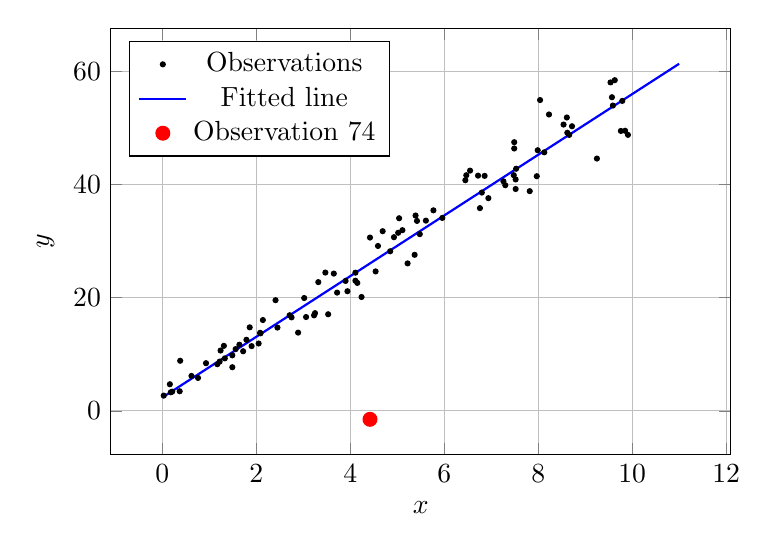
\begin{tikzpicture}
\begin{axis}[width=0.78\linewidth,height=7cm,xlabel={$x$},ylabel={$y$},grid=major,legend pos=north west]
\addplot[only marks,mark=*,mark size=0.9pt] coordinates {
(8.610,51.850)
(5.770,35.440)
(9.760,49.470)
(3.230,16.880)
(9.790,54.780)
(1.860,14.760)
(6.940,37.590)
(4.240,20.120)
(5.370,27.580)
(8.540,50.600)
(7.530,42.790)
(6.550,42.460)
(4.420,30.630)
(2.750,16.520)
(7.480,41.650)
(9.570,55.430)
(0.030,2.690)
(9.850,49.500)
(0.180,3.280)
(8.720,50.300)
(3.900,22.960)
(7.260,40.570)
(7.490,46.370)
(8.130,45.690)
(9.540,58.050)
(0.160,4.700)
(1.170,8.240)
(7.520,40.900)
(7.990,46.060)
(0.760,5.820)
(2.890,13.830)
(1.640,11.690)
(1.490,7.710)
(1.900,11.440)
(9.630,58.440)
(2.140,16.050)
(8.660,48.770)
(5.420,33.570)
(7.820,38.830)
(0.620,6.170)
(3.720,20.900)
(5.480,31.230)
(6.470,41.640)
(2.050,11.900)
(0.380,8.850)
(1.310,11.490)
(1.560,10.910)
(4.930,30.690)
(2.080,13.790)
(5.040,34.040)
(9.590,53.960)
(3.320,22.750)
(5.110,31.930)
(3.250,17.270)
(1.490,9.810)
(3.060,16.580)
(9.910,48.780)
(5.020,31.470)
(6.800,38.580)
(5.610,33.620)
(2.450,14.720)
(0.930,8.420)
(8.230,52.380)
(2.410,19.560)
(7.490,47.480)
(6.450,40.760)
(6.720,41.570)
(7.970,41.470)
(4.110,23.000)
(0.370,3.460)
(7.520,39.210)
(4.150,22.610)
(5.220,26.060)
(4.420,-1.500)
(9.250,44.590)
(1.240,10.660)
(6.760,35.830)
(1.720,10.530)
(4.690,31.750)
(7.300,39.880)
(4.590,29.140)
(5.960,34.100)
(3.470,24.440)
(5.390,34.520)
(4.110,24.420)
(3.530,17.070)
(1.330,9.270)
(0.210,3.390)
(3.020,19.940)
(3.650,24.260)
(4.850,28.200)
(4.540,24.640)
(1.220,8.700)
(2.090,13.700)
(8.620,49.150)
(1.790,12.560)
(3.940,21.140)
(2.710,16.900)
(6.860,41.530)
(8.040,54.930)
};\addlegendentry{Observations}
\addplot[domain=0:11,samples=2,thick,blue]{2.357689296+5.362331864*x};\addlegendentry{Fitted line}
\addplot[only marks,mark=*,mark size=2.5pt,red] coordinates {(4.42,-1.5)};\addlegendentry{Observation 74}
\end{axis}\end{tikzpicture}
\caption{Scatter plot with least-squares regression line.}\end{figure}
Observation 74 is unusually far below the regression line: its observed value is $-1.5$, while its fitted value is about $26.06$. It deserves investigation as a possible data error or unusual case.
\subsection{Part 1c}
After excluding observation 74, $n=99$, $\sum x_i=478.4$, $\sum y_i=2826.31$, $\sum x_i^2=3141.1176$, and $\sum x_iy_i=18093.4452$. The new estimates are $b=5.348630058$ and $a=2.702276732$. The residual and total sums of squares are $854.874742$ and $24580.337602$, respectively; hence $R^2=0.9652211961$. Removing the outlier substantially reduces unexplained variation while changing the slope and intercept only slightly.
\subsection{Part 1d}
A higher $R^2$ does not necessarily mean a better model. Adding irrelevant variables can raise $R^2$, so significance, plausible signs, and behavioural meaning also matter.
\newpage
\section{Question 2}
\subsection{Part 2a}
For zone $z$, estimate total daily shopping trips as $\hat T_z=\sum_{i\in z}w_i t_i$, where $t_i$ is surveyed household shopping trips and $w_i=H_z/n_z$ is the household weight. In zone 1, $H_1=285$, $n_1=13$, and the surveyed households made 13 shopping trips, so $\hat T_1=(285/13)(13)=285$. Appendix~\ref{app:zones} gives all 131 estimates.
\subsection{Part 2b}
All household composition and automobile variables were expanded to zonal totals. For example,
\begin{align*}
V_z&=H_z\left(\frac{1}{n_z}\sum_{i\in z}v_i\right),\\
C_z&=H_z\left(\frac{1}{n_z}\sum_{i\in z}c_i\right).
\end{align*}
where $V_z$ is estimated vehicles in the zone and $C_z$ is estimated children. Shopping-centre distance $d_z$ is a zonal attribute, not a household average. All predictors enter the regression as additive terms.
\begin{table}[H]\centering\small
\caption{Candidate zonal explanatory variables}\begin{tabular}{llcl}\toprule
Variable & Unit & Sign & Expected relationship \\\midrule
Total households $H_z$ & households/zone & $+$ & More households generate more trips.\\
Estimated vehicles $V_z$ & vehicles/zone & $+$ & Greater automobile availability supports travel.\\
Estimated children $C_z$ & children/zone & $+$ & Larger family demand may raise shopping travel.\\
Retail employment $R_z$ & jobs/zone & $+$ & Nearby retail opportunities may attract shopping.\\
Zonal population $P_z$ & persons/zone & $+$ & More residents may generate more trips.\\
Shopping distance $d_z$ & km for zone & $-$ & Longer travel distance may discourage trips.\\
\bottomrule\end{tabular}\end{table}
\subsection{Part 2c}
Ordinary least squares was estimated on 131 zones with the intercept constrained to zero to avoid a negative fixed trip count. This is a model restriction rather than a guarantee of sensible extrapolation outside the observed zone range. Each model remains linear in its coefficients. The baseline has two variables; the expanded model has five; the final model omits estimated children. The zero intercept is a modelling constraint; the fitted equations are used for the observed zone range, where all fitted trip totals are positive. Coefficients are followed by $t$-statistics in parentheses.
\begin{table}[H]\centering\small
\caption{Zonal shopping-trip regression models ($n=131$)}
\begin{tabular}{lrrr}\toprule
Term & Baseline & Expanded & Final\\\midrule
$H_z$ & 1.19717 (10.476) & 1.05776 (8.996) & 1.10252 (9.586)\\
$V_z$ & 0.21673 (1.903) & 0.22280 (2.088) & 0.24539 (2.305)\\
$C_z$ & --- & 0.51122 (1.618) & ---\\
$R_z$ & --- & 2.41230 (2.636) & 2.31142 (2.516)\\
$d_z$ & --- & $-23.29422$ ($-4.509$) & $-21.07488$ ($-4.204$)\\\midrule
Centered $R^2$ & 0.96003 & 0.96652 & 0.96582\\
Centered adjusted $R^2$ & 0.95972 & 0.96545 & 0.96501\\
\bottomrule\end{tabular}\end{table}
For comparison across these zero-intercept models, the reported centered $R^2$ is $1-\mathrm{SSE}/\sum_z(T_z-\bar T)^2$ and adjusted $R^2=1-[\mathrm{SSE}/(n-k)]/[\mathrm{SST}/(n-1)]$, where $k$ is the number of estimated slopes. Excel's zero-intercept Regression output instead reports an uncentered $R^2$; it should not be copied into this table.
\begin{align*}
\hat T_z^{\rm base}&=1.19717H_z+0.21673V_z,\\
\hat T_z^{\rm expanded}&=1.05776H_z+0.22280V_z+0.51122C_z+2.41230R_z-23.29422d_z,\\
\hat T_z^{\rm final}&=1.10252H_z+0.24539V_z+2.31142R_z-21.07488d_z.
\end{align*}
\subsection{Part 2d}
The final model retains total households, estimated zonal vehicles, retail employment, and zonal shopping-centre distance. Each coefficient has the expected sign. In the 131-zone sample, households have the strongest statistical association with shopping-trip generation ($t=9.586$). The positive vehicles coefficient is consistent with automobile availability supporting shopping travel. Retail employment has a positive association, while the negative shopping-distance coefficient is consistent with travel impedance. All four final-model slopes exceed the approximate 5\% two-sided critical magnitude of 1.98. This is a more conservative test than a one-sided test based on expected signs.

Estimated children were deliberately excluded from the final model. Its expanded-model coefficient is positive but does not reach the 5\% one-sided threshold ($t=1.618$). Adding it raises centered adjusted $R^2$ only from 0.96501 to 0.96545. The gain is small relative to the extra term. Zonal population was also available but overlaps conceptually with total households and can make the model harder to interpret. The final model therefore offers nearly the same fit with fewer predictors, plausible signs, and a nonnegative constant term. The coefficients are associations from the supplied cross-sectional sample; they should not be interpreted as causal effects without further evidence.
\subsection{Part 2e}
Zones do not provide equally reliable estimates because surveyed household counts vary from 5 to 143. Household weights scale each sample to its zone total but do not create additional observations. Zones with smaller samples generally have more sampling variability, so their estimated shopping-trip totals may be less precise.
\newpage
\section{Question 3}
\subsection{Part 3a}
For each worker and choice model, $p=\exp(V)/(1+\exp(V))$, where $V$ is the model-specific intercept plus occupation coefficient (zero for reference category G) plus the household-size coefficient times household size. The drop-off and pick-up probabilities are interpreted as conditional on a work trip for the schedule simulation.
\begin{table}[H]\centering\small\caption{Calculated probabilities for the first 10 workers}\begin{tabular}{rrrrrr}\toprule
ID & HH size & Occupation & Work & Drop-off & Pick-up\\\midrule
1 & 5 & M & 0.674955 & 0.086703 & 0.065775\\
2 & 5 & P & 0.714121 & 0.008839 & 0.007099\\
3 & 3 & M & 0.665028 & 0.249194 & 0.182075\\
4 & 2 & G & 0.680088 & 0.234495 & 0.172583\\
5 & 1 & P & 0.695441 & 0.098284 & 0.066702\\
6 & 1 & S & 0.723340 & 0.251332 & 0.183280\\
7 & 4 & M & 0.670011 & 0.150748 & 0.111262\\
8 & 2 & M & 0.660009 & 0.382940 & 0.283577\\
9 & 3 & P & 0.704867 & 0.030234 & 0.022105\\
10 & 4 & S & 0.736614 & 0.048846 & 0.038384\\
\bottomrule\end{tabular}\end{table}
\subsection{Part 3b}
The lecture's four Monte Carlo steps specialize to each binary model as follows: (1) order the two outcomes No, Yes with probabilities $1-p,p$; (2) form cumulative cutoffs $C_1=1-p$ and $C_2=1$; (3) draw $u\sim U[0,1)$; and (4) assign No when $u\le C_1$ and Yes when $u>C_1$. Thus $\mathbb{1}(u>1-p)$ is the same mapping used in the original Python code. For a coherent work schedule, the later decisions are accepted only if the worker's simulated work choice equals one:
\begin{equation*}
W_i=\mathbf 1(u_{Wi}>1-p_{Wi}),\quad
D_i=W_i\mathbf 1(u_{Di}>1-p_{Di}),\quad
U_i=W_i\mathbf 1(u_{Ui}>1-p_{Ui}).
\end{equation*}
The probabilities and random draws are retained in the table even when a later choice is suppressed. One generator was initialized once at seed 5312026 and then drew numbers in replication--worker--model order. It was not reseeded for each worker.
\begin{table}[H]\centering\scriptsize\setlength{\tabcolsep}{3pt}
\caption{Simulated choices for the first 10 workers, first replication}\begin{tabular}{r|rrr|rrr|rrr}\toprule
&\multicolumn{3}{c|}{Work}&\multicolumn{3}{c|}{Drop-off}&\multicolumn{3}{c}{Pick-up}\\
ID & $p$ & $u$ & Choice & $p$ & $u$ & Choice & $p$ & $u$ & Choice\\\midrule
1 & 0.674955 & 0.861107 & 1 & 0.086703 & 0.576648 & 0 & 0.065775 & 0.975730 & 1\\
2 & 0.714121 & 0.323168 & 1 & 0.008839 & 0.978890 & 0 & 0.007099 & 0.186039 & 0\\
3 & 0.665028 & 0.693774 & 1 & 0.249194 & 0.423755 & 0 & 0.182075 & 0.536841 & 0\\
4 & 0.680088 & 0.853909 & 1 & 0.234495 & 0.752757 & 0 & 0.172583 & 0.655007 & 0\\
5 & 0.695441 & 0.442025 & 1 & 0.098284 & 0.274669 & 0 & 0.066702 & 0.748325 & 0\\
6 & 0.723340 & 0.956901 & 1 & 0.251332 & 0.002757 & 0 & 0.183280 & 0.750242 & 0\\
7 & 0.670011 & 0.017572 & 0 & 0.150748 & 0.872260 & 0 & 0.111262 & 0.389549 & 0\\
8 & 0.660009 & 0.726032 & 1 & 0.382940 & 0.748547 & 1 & 0.283577 & 0.812622 & 1\\
9 & 0.704867 & 0.954359 & 1 & 0.030234 & 0.015693 & 0 & 0.022105 & 0.116938 & 0\\
10 & 0.736614 & 0.752265 & 1 & 0.048846 & 0.799322 & 0 & 0.038384 & 0.075893 & 0\\
\bottomrule\end{tabular}\end{table}
Worker 7 is the visible correction: the raw drop-off draw would select Yes, but the work choice is No, so the schedule's drop-off choice is set to zero.
\subsection{Part 3c}
The simulation was repeated for all 100 workers over 100 replications. If the given drop-off and pick-up probabilities are conditional on working, the expected schedule totals are $\sum_i p_{Wi}$, $\sum_i p_{Wi}p_{Di}$, and $\sum_i p_{Wi}p_{Ui}$. The products follow from the gating rule and the separately drawn random numbers. For each replication, trip choices were summed over workers; the means below average those 100 totals.
\begin{table}[H]\centering\caption{Expected and simulated schedule trip totals}\begin{tabular}{lrrr}\toprule
Model & Expected & Mean simulated & Difference\\\midrule
Work & 69.86648 & 70.08 & 0.21352\\
Drop-off & 8.68055 & 8.59 & $-0.09055$\\
Pick-up & 6.47594 & 6.25 & $-0.22594$\\\bottomrule\end{tabular}\end{table}
The small differences arise from finite Monte Carlo variation. The original ungated sums, 12.72352 and 9.49057, describe the model probabilities before the work-trip condition and are not the expected counts of feasible drop-off or pick-up trips under this schedule rule. Appendix~\ref{app:replications} lists all revised replication totals.
\subsection{Part 3d}
Workers 1 and 3 share occupation M but live in households of sizes 5 and 3. The positive household-size coefficient makes Worker 1's work-trip probability slightly higher. The negative coefficients in the drop-off and pick-up models make Worker 1's conditional probabilities for those trips lower. The difference comes from household size because their occupation category is the same.
\section*{AI/software statement}
I used Microsoft Excel for zonal aggregation and regression, Python for reproducible Monte Carlo calculations, and OpenAI Codex to help revise and check the report.
\appendix
\section{Estimated Daily Shopping Trips by Zone}\label{app:zones}
\begin{longtable}{r r r r r r}\caption{Estimated daily shopping trips for 131 zones}\\\toprule
Zone & Trips & Zone & Trips & Zone & Trips\\\midrule\endfirsthead
\toprule Zone & Trips & Zone & Trips & Zone & Trips\\\midrule\endhead
1 & 285.00000 & 45 & 281.40000 & 89 & 324.00000\\
2 & 1954.90909 & 46 & 963.40909 & 90 & 509.53846\\
3 & 308.07692 & 47 & 627.82609 & 91 & 2538.02326\\
4 & 1331.07692 & 48 & 462.48000 & 92 & 552.00000\\
5 & 631.92308 & 49 & 1508.20690 & 93 & 454.36364\\
6 & 841.40000 & 50 & 1152.89362 & 94 & 372.85714\\
7 & 623.61111 & 51 & 1638.17778 & 95 & 367.71429\\
8 & 2254.04348 & 52 & 935.52632 & 96 & 750.46154\\
9 & 290.00000 & 53 & 226.12500 & 97 & 530.63636\\
10 & 1546.41463 & 54 & 490.45455 & 98 & 556.50000\\
11 & 631.55556 & 55 & 4201.57282 & 99 & 291.20000\\
12 & 1010.46667 & 56 & 310.00000 & 100 & 2867.91045\\
13 & 2571.66667 & 57 & 453.33333 & 101 & 738.80952\\
14 & 1149.50000 & 58 & 311.25000 & 102 & 1806.00000\\
15 & 2049.35780 & 59 & 484.90000 & 103 & 207.14286\\
16 & 3204.25175 & 60 & 117.83333 & 104 & 801.89474\\
17 & 1090.55172 & 61 & 173.00000 & 105 & 650.84211\\
18 & 915.20000 & 62 & 455.40000 & 106 & 573.37500\\
19 & 378.85714 & 63 & 297.14286 & 107 & 794.41463\\
20 & 496.00000 & 64 & 2820.33898 & 108 & 278.00000\\
21 & 378.63158 & 65 & 793.00000 & 109 & 419.83333\\
22 & 912.00000 & 66 & 1810.87500 & 110 & 769.50000\\
23 & 261.30000 & 67 & 482.88000 & 111 & 262.40000\\
24 & 923.57576 & 68 & 341.88000 & 112 & 2042.04545\\
25 & 1152.75000 & 69 & 997.32258 & 113 & 626.00000\\
26 & 1667.77419 & 70 & 126.00000 & 114 & 241.00000\\
27 & 1220.42105 & 71 & 1148.94118 & 115 & 677.80645\\
28 & 525.00000 & 72 & 1832.11364 & 116 & 362.66667\\
29 & 1201.41667 & 73 & 274.30000 & 117 & 398.76923\\
30 & 1318.46154 & 74 & 384.00000 & 118 & 618.40000\\
31 & 523.81250 & 75 & 409.41176 & 119 & 568.80000\\
32 & 394.66667 & 76 & 324.00000 & 120 & 379.20000\\
33 & 1181.10000 & 77 & 667.82609 & 121 & 289.33333\\
34 & 264.00000 & 78 & 294.66667 & 122 & 5757.05263\\
35 & 1024.80000 & 79 & 459.23077 & 123 & 1144.72340\\
36 & 741.78947 & 80 & 210.00000 & 124 & 801.62500\\
37 & 490.66667 & 81 & 677.14286 & 125 & 385.00000\\
38 & 986.77419 & 82 & 2756.00000 & 126 & 2888.88889\\
39 & 690.96774 & 83 & 3163.50000 & 127 & 2558.27027\\
40 & 1315.87500 & 84 & 254.83333 & 128 & 918.18182\\
41 & 334.88889 & 85 & 682.00000 & 129 & 427.00000\\
42 & 905.00000 & 86 & 140.80000 & 130 & 1558.70000\\
43 & 218.40000 & 87 & 130.80000 & 131 & 737.43750\\
44 & 411.60000 & 88 & 474.50000 &  & \\
\bottomrule\end{longtable}
\section{Monte Carlo Simulation Code}\label{app:code}
\begin{lstlisting}[language=Python]
import numpy as np
import pandas as pd

df = pd.read_excel("Assignment_1.xlsx", sheet_name="Table_3", usecols="A:E")
h = df["Household Size: NumberOfPersons"].to_numpy()
occ = df["OccType"].astype(str).to_numpy()

intercepts = np.array([0.7092731, 0.0685556, -0.4163051])
size_coef = np.array([0.0224506, -0.6258297, -0.5755641])
occ_coef = {
    "G": [0, 0, 0],
    "M": [-0.0908422, 0.7060177, 0.6406462],
    "P": [0.0939590, -1.6591660, -1.6466180],
    "S": [0.2293679, -0.5342463, -0.5024092],
}
V = intercepts + np.array([occ_coef[o] for o in occ]) + h[:, None] * size_coef
p = 1 / (1 + np.exp(-V))

rng = np.random.default_rng(5312026)
u = rng.random((100, len(df), 3))
choices = (u > (1 - p)[None, :, :]).astype(int)
choices[:, :, 1:] *= choices[:, :, 0, None]  # Require a work trip

totals = choices.sum(axis=1)
expected = np.column_stack((p[:, 0], p[:, 0]*p[:, 1], p[:, 0]*p[:, 2])).sum(axis=0)
means = totals.mean(axis=0)
print("Expected:", expected)
print("Simulated means:", means)
print("Difference:", means - expected)
print("First 10 workers, first replication:")
for i in range(10):
    print(df.loc[i, "Person ID"], p[i], u[0, i], choices[0, i])
print("Replication totals:")
for r, row in enumerate(totals, 1):
    print(r, *row)
\end{lstlisting}
\section{Monte Carlo Replication Totals}\label{app:replications}
\begin{longtable}{r r r r r r r r}
\caption{Feasible trip totals in 100 replications}\\\toprule
Rep. & Work & Drop-off & Pick-up & Rep. & Work & Drop-off & Pick-up\\\midrule\endfirsthead
\toprule Rep. & Work & Drop-off & Pick-up & Rep. & Work & Drop-off & Pick-up\\\midrule\endhead
1 & 70 & 10 & 6 & 51 & 73 & 9 & 5\\
2 & 78 & 6 & 5 & 52 & 70 & 9 & 7\\
3 & 66 & 6 & 6 & 53 & 70 & 9 & 6\\
4 & 80 & 12 & 6 & 54 & 75 & 11 & 5\\
5 & 72 & 8 & 7 & 55 & 66 & 8 & 10\\
6 & 76 & 8 & 6 & 56 & 77 & 4 & 5\\
7 & 63 & 11 & 3 & 57 & 70 & 10 & 6\\
8 & 72 & 9 & 5 & 58 & 72 & 11 & 7\\
9 & 78 & 10 & 4 & 59 & 73 & 7 & 6\\
10 & 69 & 7 & 3 & 60 & 64 & 8 & 6\\
11 & 67 & 6 & 5 & 61 & 71 & 4 & 5\\
12 & 77 & 12 & 7 & 62 & 71 & 13 & 3\\
13 & 63 & 10 & 4 & 63 & 82 & 7 & 10\\
14 & 70 & 8 & 8 & 64 & 73 & 5 & 7\\
15 & 62 & 7 & 4 & 65 & 79 & 8 & 6\\
16 & 68 & 8 & 8 & 66 & 76 & 7 & 6\\
17 & 68 & 9 & 7 & 67 & 66 & 6 & 5\\
18 & 73 & 9 & 5 & 68 & 77 & 13 & 8\\
19 & 71 & 9 & 7 & 69 & 65 & 9 & 6\\
20 & 62 & 11 & 6 & 70 & 65 & 5 & 5\\
21 & 70 & 8 & 5 & 71 & 76 & 6 & 5\\
22 & 66 & 6 & 5 & 72 & 75 & 7 & 6\\
23 & 71 & 6 & 7 & 73 & 74 & 6 & 9\\
24 & 70 & 10 & 3 & 74 & 65 & 14 & 1\\
25 & 72 & 11 & 5 & 75 & 65 & 7 & 3\\
26 & 68 & 9 & 8 & 76 & 71 & 4 & 7\\
27 & 75 & 8 & 8 & 77 & 71 & 10 & 8\\
28 & 69 & 7 & 5 & 78 & 64 & 7 & 4\\
29 & 70 & 9 & 8 & 79 & 66 & 8 & 13\\
30 & 72 & 5 & 11 & 80 & 72 & 8 & 7\\
31 & 71 & 12 & 7 & 81 & 78 & 12 & 5\\
32 & 64 & 7 & 3 & 82 & 74 & 11 & 2\\
33 & 69 & 7 & 5 & 83 & 64 & 6 & 3\\
34 & 76 & 9 & 9 & 84 & 69 & 12 & 10\\
35 & 64 & 10 & 7 & 85 & 77 & 8 & 9\\
36 & 74 & 8 & 5 & 86 & 73 & 11 & 4\\
37 & 70 & 11 & 4 & 87 & 63 & 8 & 4\\
38 & 67 & 10 & 6 & 88 & 65 & 8 & 7\\
39 & 71 & 8 & 8 & 89 & 73 & 13 & 8\\
40 & 66 & 11 & 6 & 90 & 65 & 8 & 6\\
41 & 71 & 8 & 8 & 91 & 66 & 12 & 11\\
42 & 74 & 7 & 6 & 92 & 72 & 8 & 7\\
43 & 63 & 6 & 4 & 93 & 74 & 9 & 4\\
44 & 67 & 8 & 8 & 94 & 67 & 8 & 9\\
45 & 69 & 8 & 2 & 95 & 74 & 10 & 9\\
46 & 67 & 8 & 7 & 96 & 55 & 8 & 6\\
47 & 79 & 8 & 13 & 97 & 68 & 7 & 8\\
48 & 73 & 9 & 8 & 98 & 69 & 7 & 8\\
49 & 67 & 15 & 7 & 99 & 61 & 9 & 3\\
50 & 70 & 8 & 6 & 100 & 67 & 11 & 9\\
\bottomrule\end{longtable}
\end{document}
